\documentclass[twoside]{article}
\input{ISC18-english.sty}
%%%%%%%%%%%%%%%%%%%%%%%%%%%%  Make sure to compile twice for proper cross-references. %%%%%%%%%%%%%%%%%%%%%%%
%%%%%%% For proper display of references, compile the document twice. %%%%%%%%%%%%%%%%%%%%% 
%%%%%%%%%%%%%%% If using TeX Live, compile using pdflatex command %%%%%%%%%%%%%%%%%%%%%%%
\begin{document}
\thispagestyle{empty}
%%%%%%%%%%%%%%%%% Article title header  %%%%%%%%%%%%%%%%%%%%
\fancyhead[LE]{Bayes Estimation for Matrix-Variate Normal}
\fancyhead[RO]{H. Karamikabir}
%%%%%%%%%%%%%%%%% Article authors header   %%%%%%%%%%%%%%%%%%%%
\begin{center}
{
\includegraphics [height=25mm, width=150.3mm] {Images/isc18E}} \\
\vspace*{-1.8cm}
%\begin{center}
%\color{blue} 
%{\hspace{0.1cm}\rule{\textwidth}{1mm}}\\
%\end{center}
\vspace*{4cm}
%%%%%%%%%%%%%%%%% Article title  %%%%%%%%%%%%%%%%%%%%
{\Large \bf Shrinkage Bayes Estimation for Matrix-Variate Normal Mean Matrix under Balanced Loss Function }\\
%%%%%%%%%%%%%%%%% Article authors and affiliations %%%%%%%%%%%%%%%%%%%%
{\bf
Hamid Karamikabir\footnote[1]{{\bf Corresponding Author:} {\tt h\_karamikabir@pgu.ac.ir }}  \\
Department of Statistics, Faculty of Intelligent Systems Engineering and Data Science, Persian Gulf University, Bushehr, Iran\\}
\end{center}
\rule{\textwidth}{0.2mm}\\
%%%%%%%%%%%%%%%%% Article abstract  %%%%%%%%%%%%%%%%%%%%
\noindent{\bf Abstract:}\\
We study Bayesian estimation of the mean matrix in a matrix-variate normal distribution with known covariances and a conjugate prior. Under a balanced matrix composite loss function, we derive the Bayes estimator as a convex combination of the posterior mean and the observed data, controlled by a shrinkage parameter $\omega \in [0,1]$. The posterior mean formula $\Theta_n = \frac{1}{2}(\Theta_0 + X)$ is established. A simulation study using non-diagonal AR(1) covariances confirms the theoretical findings, showing that the optimal $\omega$ lies strictly between zero and one under high noise, with the optimal estimator achieving $38.4\%$ MSE reduction over the posterior mean. Performance is evaluated using MSE, PSNR, and SSIM metrics.
 
\noindent{\bf Keywords:} 
Balanced loss function, Bayes estimator,  Image denoising, Matrix-variate normal distribution,  Shrinkage estimation. \\
\noindent{\bf Mathematics Subject Classification (2010):} $62J07$, $62F15$.\\
\hspace{1cm}\rule{\textwidth}{0.2mm}\\

%%%%%%%%%%%%%%
%%%%%%%%%%%%%%%%%%%%%%%%%%%%%%%%%
%%%%%%%%%%%%%%%%%%%%%%%%%%%%%%%%%
\section{Introduction}

The study of matrix-variate distributions is fundamental in statistics, machine learning, and Bayesian inference. In many applications, data naturally appear as matrices (e.g., images, economic panels, gene expression). Modeling such data requires frameworks that capture dependencies across both rows and columns. 
The matrix-variate normal distribution, denoted $X \sim \mathcal{MN}(\Theta, \Sigma_p, \Sigma_n)$, extends the multivariate normal by introducing separate covariance matrices for rows and columns, enabling row-wise and column-wise correlations. 

In the Bayesian framework, determining the posterior distribution of the mean matrix $\Theta$ is of particular interest. Conjugacy ensures analytical tractability. For the matrix-variate normal model, the conjugate prior for $\Theta$ is the normal-Wishart distribution. Specifically, $\Theta \sim \mathcal{MN}(\Theta_0, \Sigma_p, \Sigma_n)$, where $\Theta_0$ is the prior mean. 
In statistical estimation, the choice of loss function is crucial. For the mean matrix $\Theta$, weighted and matrix-based loss functions can incorporate dependencies and heteroscedasticity. In this paper, we consider the balanced matrix composite loss function for estimating $\Theta$.
\begin{dfn}
For covariance matrices $\Sigma_p$ and $\Sigma_n$, the balanced matrix composite loss is
    \begin{equation}
    L_{BM}(\hat{\Theta}, \Theta) = (1-\omega) \mathrm{tr}\Big( (\hat{\Theta} - \Theta)^\top \Sigma_p^{-1} (\hat{\Theta} - \Theta) \Sigma_n^{-1} \Big)
   + \omega  \mathrm{tr}\Big( (\hat{\Theta} - \delta_0(X))^\top \Sigma_p^{-1} (\hat{\Theta} - \delta_0(X)) \Sigma_n^{-1} \Big),
     \end{equation}
where $\delta_0(X)$ is the target estimator matrix.
\end{dfn}
The history of matrix estimation, especially for high-dimensional data, is extensive. Early Bayesian approaches include \cite{tsu2010}, who estimated the mean matrix in elliptically contoured distributions using shrinkage priors. Recent advances by  \cite{yua} provided generalized Bayes estimators with closed-form solutions.
 \cite{kar24} extended this to elliptically contoured distributions under a balanced loss function. \cite{zin} developed a class of Bayes minimax estimators under quadratic loss. \cite{kar25} refined wavelet thresholding with new SURE thresholds under reflected normal balanced loss. Finally, \cite{bat} proposed Bayesian shrinkage wavelet estimators combining shrinkage with SURE-based thresholds.
%%%%%%%%%%%%%%%%%%%%%%%%%%%%%%%%%
%%%%%%%%%%%%%%%%%%%%%%%%%%%%%%%%%
\section{Main Result}
This section establishes the posterior distribution for the matrix-variate normal distribution with a conjugate prior for the mean matrix. We assume that our observed data follows a matrix-variate normal distribution, $X \sim \mathcal{MN}(\Theta, \Sigma_p, \Sigma_n)$, and our goal is to compute the posterior distribution of the mean matrix $\Theta$ after observing the data. Suppose that $X \sim \mathcal{MN}(\Theta, \Sigma_p, \Sigma_n)$ where $X$ is a $p \times n$ matrix of observations and $\Theta$ is the matrix mean. 
It is worth noting that the classical multivariate normal distribution is a special case of the matrix-variate normal distribution. Specifically, when the observed data matrix $X$ reduces to a vector, i.e., when either the number of rows $p = 1$ or the number of columns $n = 1$, the matrix-variate normal distribution simplifies to the multivariate normal distribution.
Thus, the matrix-variate normal distribution generalizes the multivariate normal by allowing separate covariance structures for rows and columns, capturing dependencies in both directions.

For the mean matrix $\Theta$, a conjugate prior is given by $\Theta \sim \mathcal{MN}(\Theta_0, \Sigma_p, \Sigma_n)$, where $\Theta_0$ is the prior mean for $\Theta$.
To compute the posterior distribution for $\Theta$, we start with the likelihood function and the prior distribution. The likelihood function of the matrix-variate normal distribution is given by:
\begin{eqnarray}\label{like}
f(X \mid \Theta, \Sigma_p, \Sigma_n) = 
\frac{
\exp\left(-\frac{1}{2} \mathrm{tr} \left( \Sigma_p^{-1} (X - \Theta) \Sigma_n^{-1} (X - \Theta)^T \right)\right)
}{
(2\pi)^{\frac{np}{2}} |\Sigma_p|^{\frac{n}{2}} |\Sigma_n|^{\frac{p}{2}}
}
\end{eqnarray}
Similarly, the prior for $\Theta \sim \mathcal{MN}(\Theta_0, \Sigma_p, \Sigma_n)$ is:
\[
\pi(\Theta \mid \Sigma_p, \Sigma_n) = 
\frac{
\exp\left(-\frac{1}{2} \mathrm{tr} \left( \Sigma_p^{-1} (\Theta - \Theta_0) \Sigma_n^{-1} (\Theta - \Theta_0)^T \right)\right)
}{
(2\pi)^{\frac{np}{2}} |\Sigma_p|^{\frac{n}{2}} |\Sigma_n|^{\frac{p}{2}}
}
\]
Because the prior and likelihood are conjugate, the posterior distribution of $\Theta$ given $X$ is also matrix-variate normal:
\[
\pi(\Theta \mid X, \Sigma_p, \Sigma_n) \propto f(X \mid \Theta, \Sigma_p, \Sigma_n) \cdot \pi(\Theta \mid \Sigma_p, \Sigma_n)
\]
Multiplying and combining the exponent terms, the posterior distribution is as follows:
\begin{eqnarray*}
&\propto & 
\exp\left(-\frac{1}{2} \mathrm{tr} \left[ 
\Sigma_p^{-1} (X - \Theta) \Sigma_n^{-1} (X - \Theta)^{T} 
+ \Sigma_p^{-1} (\Theta - \Theta_0) \Sigma_n^{-1} (\Theta - \Theta_0)^{T}
\right] \right) \\
&=& 
\exp\left(-\frac{1}{2} \mathrm{tr} \Big[
\Sigma_p^{-1} 
\Big( 2\,\Theta \Sigma_n^{-1} \Theta^{T} - \Theta \Sigma_n^{-1} (X + \Theta_0)^{T}
- (X + \Theta_0) \Sigma_n^{-1} \Theta^{T}
+ X \Sigma_n^{-1} X^{T} + \Theta_0 \Sigma_n^{-1} \Theta_0^{T}
\Big) \Big] \right).
\end{eqnarray*}
By completing the square in $\Theta$, the quadratic form above can be rewritten as
\[
\mathrm{tr}\!\left[
\Sigma_p^{-1}
\left( 2(\Theta - \tfrac{1}{2}(X+\Theta_0)) \Sigma_n^{-1} (\Theta - \tfrac{1}{2}(X+\Theta_0))^{T}
\right) \right] + \text{constant terms independent of } \Theta.
\]
Hence, the posterior distribution of $\Theta$ is matrix-variate normal $
\Theta \mid X, \Sigma_p, \Sigma_n 
\sim \mathcal{MN}(\Theta_n, \Sigma_p^*, \Sigma_n)$, where $\Theta_n = \frac{1}{2}(\Theta_0 + X)$. Thus, the posterior mean is the precision-weighted average of the prior mean and the observed data matrix.
\subsection{The Bayes estimator for the mean matrix $\Theta$}
This subsection focuses on deriving the Bayes estimator for the mean matrix $\Theta$ under different loss functions. Specifically, we consider balanced Frobenius loss functions and balanced matrix composite loss functions. We provide explicit formulas for the Bayes estimators and discuss their dependence on the posterior mean and the observed data matrix.
Consider the matrix-variate normal likelihood $X \mid \Theta, \Sigma_p, \Sigma_n \sim \mathcal{MN}(\Theta, \Sigma_p, \Sigma_n)$, with the conjugate prior $\Theta \sim \mathcal{MN}(\Theta_0, \Sigma_p, \Sigma_n)$.
\begin{thm}\label{t32}
Let $X \in \mathbb{R}^{n \times p}$ be the observed data matrix, and suppose the unknown parameter matrix $\Theta \in \mathbb{R}^{n \times p}$ has the posterior distribution $\Theta \mid X \sim \mathcal{MN}_{n \times p}(\Theta_n, \Sigma_p, \Sigma_n)$. Then, under the loss function $L_{BM}(\hat{\Theta}, \Theta)$ with the target estimator matrix $\delta_0(X)= X$, the Bayes estimator $\hat{\Theta}^{\mathrm{B}}$ minimizing the posterior expected loss is given by $\hat{\Theta}^{\mathrm{B}} = (1-\omega) \Theta_n + \omega X$.
\end{thm}
\begin{proof}
The posterior expected loss is
\begin{eqnarray*}
R(\hat{\Theta}) &=& \mathbb{E}_{\Theta \mid X}[L_{BM}(\hat{\Theta}, \Theta)] = (1-\omega) \mathbb{E}_{\Theta \mid X}\left[\mathrm{tr}\left((\hat{\Theta} - \Theta)^\top \Sigma_p^{-1} (\hat{\Theta} - \Theta) \Sigma_n^{-1}\right)\right] \\
&&+ \omega \, \mathrm{tr}\left((\hat{\Theta} - X)^\top \Sigma_p^{-1} (\hat{\Theta} - X) \Sigma_n^{-1}\right).
\end{eqnarray*}

Since $X$ is fixed, the second term is constant with respect to $\Theta$. For the first term, we write $\hat{\Theta} - \Theta = (\hat{\Theta} - \Theta_n) + (\Theta_n - \Theta)$. Expanding the quadratic form and taking expectation gives
\begin{eqnarray*}
&&\mathbb{E}_{\Theta \mid X}\left[\mathrm{tr}\left((\hat{\Theta} - \Theta)^\top \Sigma_p^{-1} (\hat{\Theta} - \Theta) \Sigma_n^{-1}\right)\right] \\
&& =\mathrm{tr}\left((\hat{\Theta} - \Theta_n)^\top \Sigma_p^{-1} (\hat{\Theta} - \Theta_n) \Sigma_n^{-1}\right) \\
&& \quad + 2 \, \mathbb{E}_{\Theta \mid X}\left[\mathrm{tr}\left((\hat{\Theta} - \Theta_n)^\top \Sigma_p^{-1} (\Theta_n - \Theta) \Sigma_n^{-1}\right)\right] \\
&& \quad + \mathbb{E}_{\Theta \mid X}\left[\mathrm{tr}\left((\Theta_n - \Theta)^\top \Sigma_p^{-1} (\Theta_n - \Theta) \Sigma_n^{-1}\right)\right].
\end{eqnarray*}
The cross-term vanishes because $\mathbb{E}_{\Theta \mid X}[\Theta_n - \Theta] = 0$, and the last term is the posterior variance, which is independent of $\hat{\Theta}$. Thus, we have:
\[
\mathbb{E}_{\Theta \mid X}\left[\mathrm{tr}\left((\hat{\Theta} - \Theta)^\top \Sigma_p^{-1} (\hat{\Theta} - \Theta) \Sigma_n^{-1}\right)\right] = \mathrm{tr}\left((\hat{\Theta} - \Theta_n)^\top \Sigma_p^{-1} (\hat{\Theta} - \Theta_n) \Sigma_n^{-1}\right) + C_1,
\]
where $C_1$ is a constant.

Ignoring terms independent of $\hat{\Theta}$, minimizing $R(\hat{\Theta})$ reduces to minimizing
\[
F(\hat{\Theta}) = (1-\omega) \, \mathrm{tr}\left((\hat{\Theta} - \Theta_n)^\top \Sigma_p^{-1} (\hat{\Theta} - \Theta_n) \Sigma_n^{-1}\right) + \omega \, \mathrm{tr}\left((\hat{\Theta} - X)^\top \Sigma_p^{-1} (\hat{\Theta} - X) \Sigma_n^{-1}\right).
\]
To find the minimizer, we compute the derivative of $F(\hat{\Theta})$ with respect to $\hat{\Theta}$. Using matrix calculus identities
\[
\frac{\partial F(\hat{\Theta})}{\partial \hat{\Theta}} = 2(1-\omega) \, \Sigma_p^{-1} (\hat{\Theta} - \Theta_n) \Sigma_n^{-1} + 2\omega \, \Sigma_p^{-1} (\hat{\Theta} - X) \Sigma_n^{-1}.
\]
Setting the derivative to zero gives $(1-\omega) \, \Sigma_p^{-1} (\hat{\Theta} - \Theta_n) \Sigma_n^{-1} + \omega \, \Sigma_p^{-1} (\hat{\Theta} - X) \Sigma_n^{-1} = 0$. Since $\Sigma_p^{-1}$ and $\Sigma_n^{-1}$ are positive definite and hence invertible, we can multiply both sides on the left by $\Sigma_p$ and on the right by $\Sigma_n$, yielding 
$
(1-\omega)(\hat{\Theta} - \Theta_n) + \omega (\hat{\Theta} - X) = 0,
$
which gives the unique solution $\hat{\Theta}^{\mathrm{B}} = (1-\omega) \Theta_n + \omega X$. The uniqueness follows from the strict convexity of $F(\hat{\Theta})$.
\end{proof}
Note that $\hat{\Theta}^{\mathrm{B}} = (1-\omega) \, \Theta_n + \omega \, X, \quad \text{with} \quad \Theta_n = \frac{1}{2} (\Theta_0 + X)$. Substituting $\Theta_n$ gives
\[
\hat{\Theta}^{\mathrm{B}} = (1-\omega) \frac{1}{2} (\Theta_0 + X) + \omega X
= \frac{1-\omega}{2} \Theta_0 + \frac{1-\omega}{2} X + \omega X
= \frac{1-\omega}{2} \Theta_0 + \frac{1+\omega}{2} X.
\]
Therefore, the Bayes estimator has form
\begin{eqnarray}\label{eq:Bayes-conv}
\hat{\Theta}^{\mathrm{B}} = \frac{1-\omega}{2} \Theta_0 + \frac{1+\omega}{2} X.	
\end{eqnarray}

\begin{cor}
In accordance with Theorem~\ref{t32}, the explicit forms of the Bayes estimators for the parameter matrix $\Theta$ are as follows:
\begin{enumerate}
    \item In the limiting case $\omega \to 0$, the Bayes estimator converges to the posterior mean $\Theta_n$, i.e., $\lim_{\omega \to 0} \hat{\Theta}^{\mathrm{B}} = \Theta_n$.
    \item In the limiting case $\omega \to 1$, the Bayes estimator converges to the observed data matrix $X$, and we have $\lim_{\omega \to 1} \hat{\Theta}^{\mathrm{B}} = X$.
    \item For any fixed $\omega \in (0,1)$, the Bayes estimator is a convex combination of $\Theta_n$ and $X$ as presented in \eqref{eq:Bayes-conv}.
\end{enumerate}
\end{cor}
%%%%%%%%%%%%%%%%%%%%%%%%
%%%%%%%%%%%%%%%%%%%%%%%%
%%%%%%%%%%%%%%%%%%%%%%%%
\section{Simulation Study}
In this section, we present a simulation study to validate the theoretical results derived in Section 3. The simulation aims to verify the posterior distribution of the mean matrix $\Theta$, evaluate the performance of the Bayes estimator under the balanced matrix composite loss function, and investigate the behavior of the optimal shrinkage parameter $\omega$.

We consider a $p \times n$ matrix-variate normal model with $p = 32$ rows and $n = 32$ columns. The true mean matrix $\Theta_{\text{true}}$ is constructed as a smooth two-dimensional pattern using sinusoidal functions, resulting in an image with pixel values ranging approximately from $-15$ to $115$. The prior mean is set to a constant matrix $\Theta_0 = 60 \cdot \mathbf{1}_{p \times n}$, representing a simple non-informative prior that differs substantially from the true mean.
For the covariance matrices, we employ a non-diagonal AR(1) structure defined as $[\Sigma]_{ij} = \sigma^2 \rho^{|i-j|}$. The correlation parameters are set to $\rho_p = \rho_n = 0.5$ to introduce moderate dependence between rows and columns, while the variance parameters are set to $\sigma^2_p = \sigma^2_n = 15$ to create substantial noise in the observed data. The trace of each covariance matrix is $480$, indicating significant variability.

The observed data matrix $X$ is generated from $X \sim \mathcal{MN}(\Theta_{\text{true}}, \Sigma_p, \Sigma_n)$. The posterior mean is $\Theta_n = \frac{1}{2}(\Theta_0 + X)$. The Bayes estimator family from Theorem~\ref{t32}  is given by $\hat{\Theta}^{\mathrm{B}}(\omega) = \frac{1-\omega}{2}\Theta_0 + \frac{1+\omega}{2}X$ for $\omega \in [0,1]$. We evaluate this estimator for $20$ equally spaced $\omega$ values. To assess performance, we compute three metrics directly on the raw data without normalization: Mean Squared Error (MSE), Peak Signal-to-Noise Ratio (PSNR), and Structural Similarity Index (SSIM).

The numerical results of the simulation are presented in Tables~\ref{tab:estimators} and~\ref{tab:omega_performance}, and the visual comparison of estimators is shown in Figure~\ref{fig:estimators}.
\begin{table}[htbp]
\centering
\caption{Performance of the Bayes estimator for selected $\omega$ values.}
\label{tab:omega_performance}
\begin{tabular}{|c|c|c|c|}
\hline
$\omega$ & \textbf{MSE} & \textbf{PSNR (dB)} & \textbf{SSIM} \\
\hline
0.000 & 282.6639 & 17.75 & 0.7187 \\
0.263 & 212.0946 & 19.00 & 0.7893 \\
0.526 & 177.6724 & 19.77 & 0.8238 \\
0.789 & 179.3971 & 19.72 & 0.8318 \\
1.000 & 206.8027 & 19.11 & 0.8245 \\
\hline
\end{tabular}
\end{table}
The simulation results confirm our theoretical findings. A key observation from Table~\ref{tab:omega_performance} is the existence of an interior optimal $\omega$ strictly between $0$ and $1$. As $\omega$ increases from $0$ to approximately $0.6$, both PSNR and SSIM improve while MSE decreases. Beyond this optimal region, further increasing $\omega$ leads to performance degradation. This U-shaped behavior demonstrates that neither the posterior mean ($\omega = 0$) nor the raw data ($\omega = 1$) alone provides the best estimate; instead, an optimal convex combination achieves superior performance.
The optimal $\omega$ values based on different criteria are $\omega^* = 0.632$ (based on PSNR and MSE) and $\omega^* = 0.737$ (based on SSIM). The close agreement between these criteria validates the robustness of our findings. The optimal Bayes estimator achieves an MSE of $174.02$, which represents a $38.4\%$ reduction compared to the posterior mean (MSE $= 282.66$) and a $15.8\%$ reduction compared to the observed data (MSE $= 206.80$).

Figure~\ref{fig:estimators} provides visual confirmation of these results. Panel (a) shows the true image $\Theta_{\text{true}}$ with its smooth sinusoidal pattern. Panel (b) displays the constant prior mean $\Theta_0 = 60$, which is clearly far from the truth as reflected by its poor metrics (MSE $= 880.49$, PSNR $= 12.82$ dB). Panel (c) presents the observed data $X$ containing substantial noise due to the high variance setting ($\sigma^2=15$), making the underlying pattern difficult to discern. Panel (d) shows the posterior mean $\Theta_n$ ($\omega=0$), which smooths the noise but remains somewhat blurry with MSE $= 282.66$. Panel (e) illustrates the optimal Bayes estimator at $\omega^* = 0.632$, which achieves a better balance by preserving more structural details while effectively reducing noise, resulting in the best MSE ($174.02$) and PSNR ($19.86$ dB). Finally, panel (f) displays the evolution of MSE, PSNR, and SSIM as functions of $\omega$, clearly illustrating the peak performance near $\omega = 0.63$ and the U-shaped behavior of the error metrics.
\begin{figure}[ht]
\begin{center}
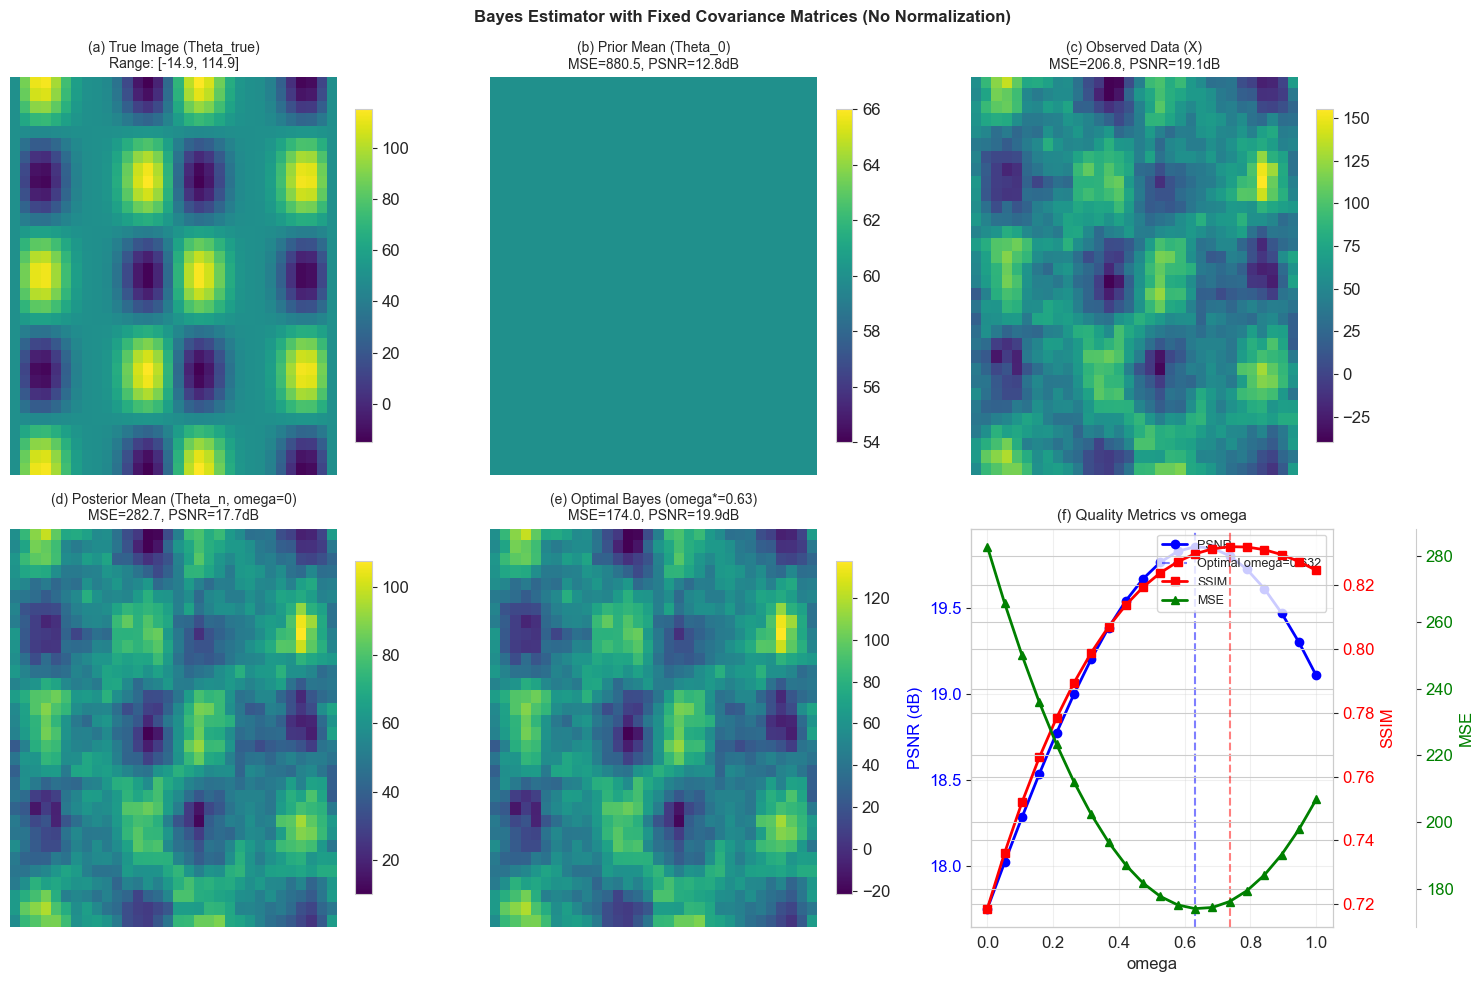
\includegraphics[scale=0.4]{Images/output.png}
\vspace{-0.2cm}
\caption{\footnotesize{Comparison of different estimators. (a) True image $\Theta_{\text{true}}$, (b) Prior mean $\Theta_0$, (c) Observed data $X$, (d) Posterior mean $\Theta_n$ ($\omega=0$), (e) Optimal Bayes estimator ($\omega^*=0.632$), (f) Quality metrics versus $\omega$ showing MSE, PSNR and SSIM.}}
\label{fig:estimators}
\end{center}
\end{figure}
Table~\ref{tab:estimators} summarizes the performance of the reference estimators. The prior mean performs poorly (MSE $= 880.49$, SSIM $= 0.033$) as expected, since it is chosen to be substantially different from the true mean. The observed data shows moderate performance (PSNR $= 19.11$ dB, SSIM $= 0.8245$), while the posterior mean improves upon the prior but remains inferior to the observed data. The optimal Bayes estimator outperforms both, achieving the highest PSNR ($19.86$ dB) and SSIM ($0.8319$), and the lowest MSE ($174.02$).
\begin{table}[htbp]
\centering
\caption{Quality metrics for different estimators.}
\label{tab:estimators}
\begin{tabular}{|l|c|c|c|}
\hline
\textbf{Estimator} & \textbf{MSE} & \textbf{PSNR (dB)} & \textbf{SSIM} \\
\hline
Prior Mean ($\Theta_0$) & 880.4871 & 12.82 & 0.0330 \\
Observed Data ($X$, $\omega=1$) & 206.8027 & 19.11 & 0.8245 \\
Posterior Mean ($\Theta_n$, $\omega=0$) & 282.6639 & 17.75 & 0.7187 \\
Optimal Bayes ($\omega^*=0.632$) & 174.0246 & 19.86 & 0.8319 \\
\hline
\end{tabular}
\end{table}
\section*{Discussion and Conclusion}  
In this paper, we derived the Bayes estimator for the mean matrix under a matrix-variate normal model with conjugate prior and balanced matrix composite loss. Simulation results confirmed that the optimal shrinkage parameter $\omega$ lies strictly between zero and one in high-noise scenarios, validating that both prior information and observed data contribute meaningfully to estimation.

 
%The conclusion of the article should be presented in a maximum of 3 or 4 lines.
%\section*{Acknowledgments}   
%If you wish to include acknowledgments, this section should appear before the references.
%%%%%%%%%%%%%%%%%%%%%%%%%%%%%%%  %%%%%%%%%%%%%%%%%%%%%%%%%%%%%%%%%
\begin{thebibliography}{9}
%\bibitem[Craik (2005)]{Craik:2005}
%Craik A.D.D. (2005), Prehistory of Fa\`{a} di Bruno's formula, {\it The American Mathematical Monthly} 112, 2,  119-130.
%\bibitem[Feller (1972)]{Feller:1972} 
%Feller W. (1972), {\it An introduction to probability theory and its applications,} New York, John Wiley.
%\bibitem[Genest and  Rivest (1993)]{Genest:Rivest:1993}
%Genest C. and  Rivest L.P. (1993), Statistical inference
%procedures for bivariate Archimedean copulas, {\it J. Amer.
%Statist. Assoc.} 88,  1034 - 1043.
%
%\bibitem[Li et al. (2015)]{LZ15}
%Li K., Zheng W. and Ai M. (2015), Optimal designs for the proportional interference model, {\it The Annals of Statistics}, 43(4), 1596-1616.
%%%%%%%%%%%%%%%%%%%%%%%%%%%%%%%%%%%%%%%%
\bibitem[Tsukuma (2010)]{tsu2010}
Tsukuma H. (2010), Shrinkage priors for Bayesian estimation of the mean matrix in an elliptically contoured distribution, {\it Journal of Multivariate Analysis} 101(6), 1483-1492. %%%%%%%%%%%%%%%

\bibitem[Yuasa and Kubokawa (2023)]{yua}
Yuasa R. and Kubokawa T. (2023), Generalized Bayes estimators with closed forms for the normal mean and covariance matrices, {\it Journal of Statistical Planning and Inference} 222, 182-194. 

\bibitem[Karamikabir (2024)]{kar24}
Karamikabir H. (2024), Wavelet Shrinkage Estimation for Mean Matrix of Matrix-Variate Elliptically Contoured Distributions, {\it Journal of Statistical Theory and Practice} 18(2), 23. %%%%%%%%%%%%%%%

\bibitem[Zinodiny and Nadarajah (2024)]{zin}
Zinodiny S. and Nadarajah S. (2024), A New Class of Bayes Minimax Estimators of the Mean Matrix of a Matrix Variate Normal Distribution, {\it Mathematics} 12(7), 1098. %%%%%%%%%%%%%%%

\bibitem[Karamikabir et al.  (2025)]{kar25}
Karamikabir H., Sanati A. and Hamedani G.G. (2025), Low and high dimensional wavelet thresholds for matrix-variate normal distribution, {\it Communications in Statistics-Simulation and Computation} 54(7), 2742-2761.
%%%%%%%%%%%%%%%

\bibitem[Batvandi et al.  (2025)]{bat}
Batvandi Z., Afshari M. and Karamikabir H. (2025), Bayesian shrinkage wavelet estimation of mean matrix of the matrix variate normal distribution with application in de-noising, {\it Computational and Applied Mathematics} 44(1), 43. %%%%%%%%%%%%%%%



\end{thebibliography}
 \end{document}

